\documentclass[12pt]{article}
\usepackage{amsmath, amsthm,amssymb}
\usepackage{graphicx}

\newcommand{\BEASTVersion}{2.2.x}
\newcommand{\TracerVersion}{1.6}
\newcommand{\FigTreeVersion}{1.4.2}


\newcommand{\lra}[1]{\langle #1 \rangle}

% turnover = birth / death
\newcommand{\turnover}{\nu}

% sampling proportion = \psi / \psi + \mu
\newcommand{\fosp}{s}

\newcommand*\rot{\rotatebox{90}}
\newcommand*\OK{\ding{51}}


\pagestyle{empty}

\sloppy

%\bibliographystyle{abbrv}

\title{Dating with FBD model tutorial}

\author{Alexandra Gavryushkina}

\date{}

\begin{document}

\maketitle


\section{Introduction}

The tutorial illustrates how to use the BEAST software to co-estimate gene phylogenies and associated divergence times using fossil evidence and the fossilised birth-death (FBD) model. 
The data required for such an analysis:

\begin{itemize}

\item Molecular data of extant species. 

\item Occurrence dates (or ranges) of fossil samples.

\item Prior knowledge about the parameters of the FBD model. It could be a known proportion of sampled extant species, for example.

\item Optionally, you may introduce monophyletic constraints on the phylogeny. 

\end{itemize}

You will need the following software at your disposal: 

\begin{itemize}

\item {\bf BEAST} - this package contains the BEAST program, BEAUti, TreeAnnotator and other utility programs. This tutorial is written for BEAST v{\BEASTVersion}. It is available for download from \texttt{http://www.beast2.org/}.  A sampled ancestor (SA) package available for this version supports sampled ancestor trees and FBD model. The package can be installed through the package manager in BEAUti.  
\item {\bf Tracer} - this program is used to explore the output of BEAST (and other Bayesian MCMC programs). It graphically and
quantitively summarizes the distributions of continuous parameters and provides diagnostic information. At the time of
writing, the current version is v{\TracerVersion}. It is available for download from\\*\texttt{http://tree.bio.ed.ac.uk/software/}.
\item {\bf FigTree} - this is an application for displaying and printing molecular phylogenies, in particular those obtained using
BEAST. At the time of writing, the current version is v{\FigTreeVersion}. It is available for download from \texttt{http://tree.bio.ed.ac.uk/software/}.
\end{itemize}
And we assume that you are familiar with basics of using BEAUti and BEAST. 

\section{Preparing the XML file}

Having BEAST and SA package installed and sequence data of extant species together with empty sequences of fossil samples in a NEXUS file we can start preparing an XML file - the file which contain the specification of the analysis. First of all we need to upload the NEXUS file to BEAUti. In this tutorial, we use an example nexus file, bears.nex, which is available from the {\tt examples/nexus/} directory for Mac and Linux and  {\tt examples\textbackslash nexus\textbackslash} for Windows inside the directory where SA package was installed. The package manager installs packages to \\
{\tt /Users/<YourName>/Library/Application Support/BEAST/2.2/} on Mac, \\
{\tt /home/<YourName>/.beast/2.2/} on Linux, and \\
{\tt Users\textbackslash<YourName>\textbackslash BEAST\textbackslash 2.2\textbackslash} on Windows.

%\begin{figure}	
%\centering
%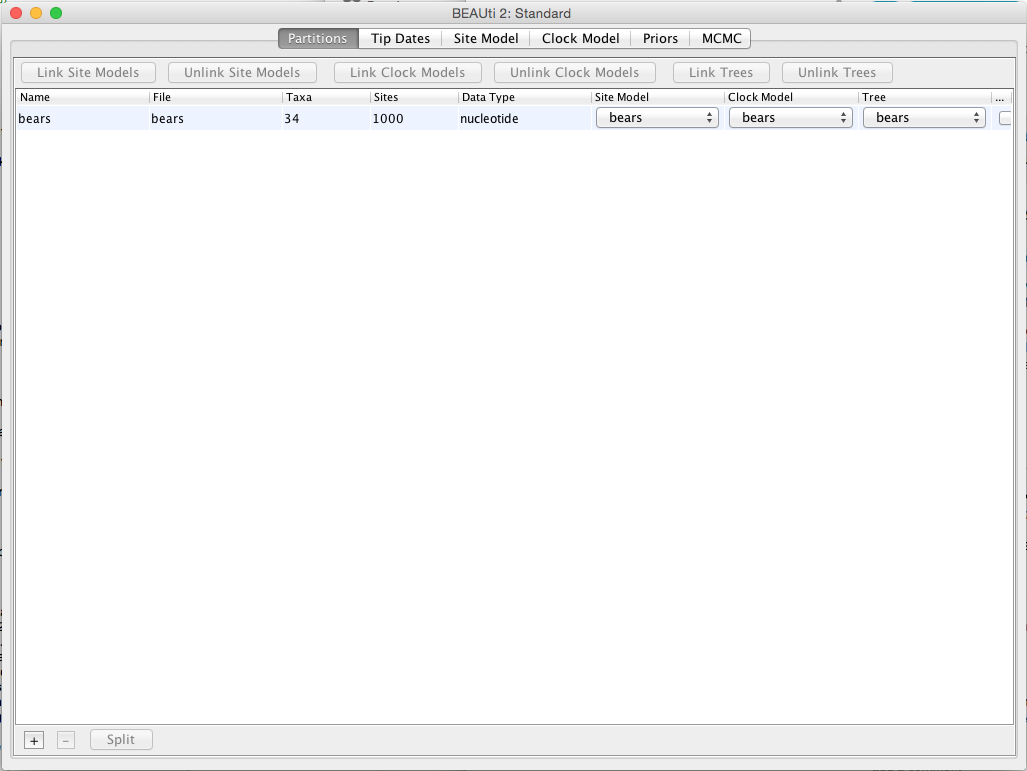
\includegraphics[width=\textwidth]{figures/AlignmentViewer}
%\caption{The {\bf Partition} panel in BEAUti with a loaded alignment.\label{fig:alignmentViewer}}
%\label{fig:BEAUti_ImportNexus}
%\end{figure}
The example file contains an alignment of a single gene of ten extant species and 24 fossil samples (each site in the fossil sequences is a gap).   
After loading the alignment you may need to link trees and clock models if this is an alignment of different genes. 

The next step is to specify the ages in the {\bf Tip Dates} panel. Tick the `Use tip dates' box. Then choose the right options in `Dates specified as' section. We choose `years' (the ages are actually given in My) and `Before the present' options.  Click on the `Guess' button to load the dates from a separate file or extract the dates from taxon names or type in the dates directly to the cells of the table.  In the example NEXUS file, the ages are included in the names of the taxa. So we choose `use everything after last \_' option to extract the dates (see Figure \ref{fig:tipDates}).

\begin{figure}	
\centering
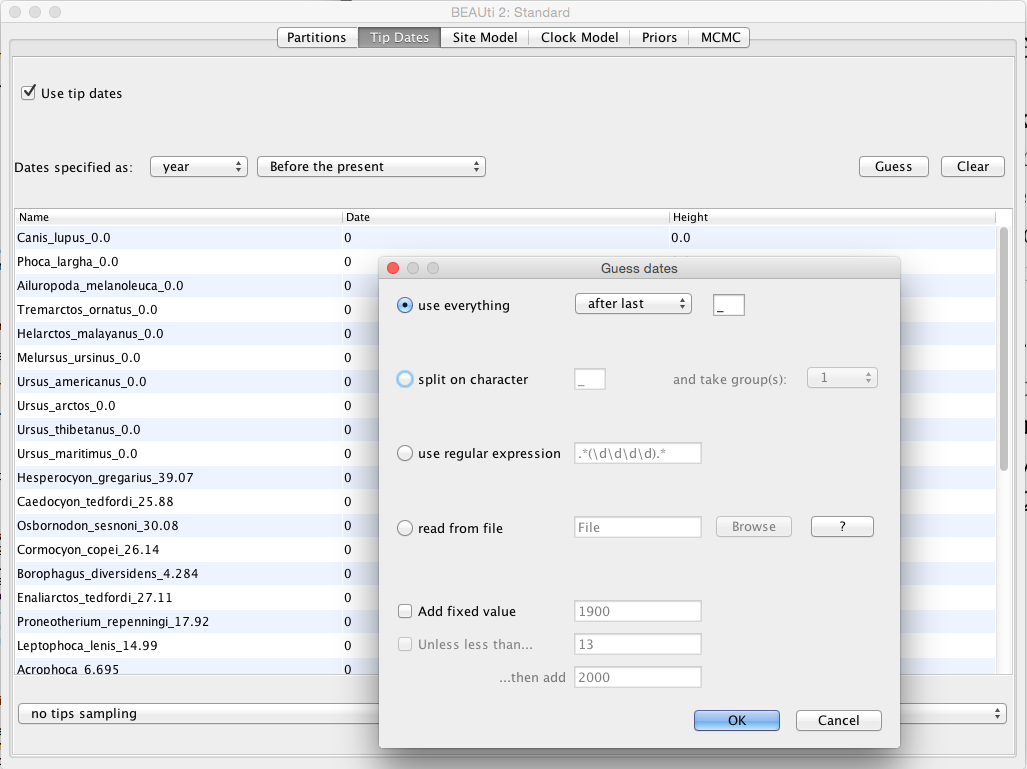
\includegraphics[width=\textwidth]{figures/TipDates}
\caption{The {\bf Tip Dates} panel in BEAUti. Select `Use tip dates' and then 'Dates specified as' options. Then extract the dates from the taxon labels by clicking on `Guess' button.\label{fig:tipDates}}
\label{fig:BEAUti_ImportNexus}
\end{figure}
It is also possible to specify the age ranges however BEAUti does not support this option. If you want to do this then finish the XML specification in BEAUti and add the ranges manually.  See bears\_ranges.xml example file in {\tt examples/} folder in the SA package directory as an example, the relevant part . Note that you still need to specify the ages in BEAUti. These ages should be within the ranges and will be used as initial values. 

Further we need to specify site and clock models. We leave the default site model and choose the `Relaxed Clock Log Normal' model with all default settings. Next we choose the `Fossilised Birth Death Model' as the tree prior distribution (see Figure \ref{fig:FBDmodel}).

\begin{figure}	
\centering
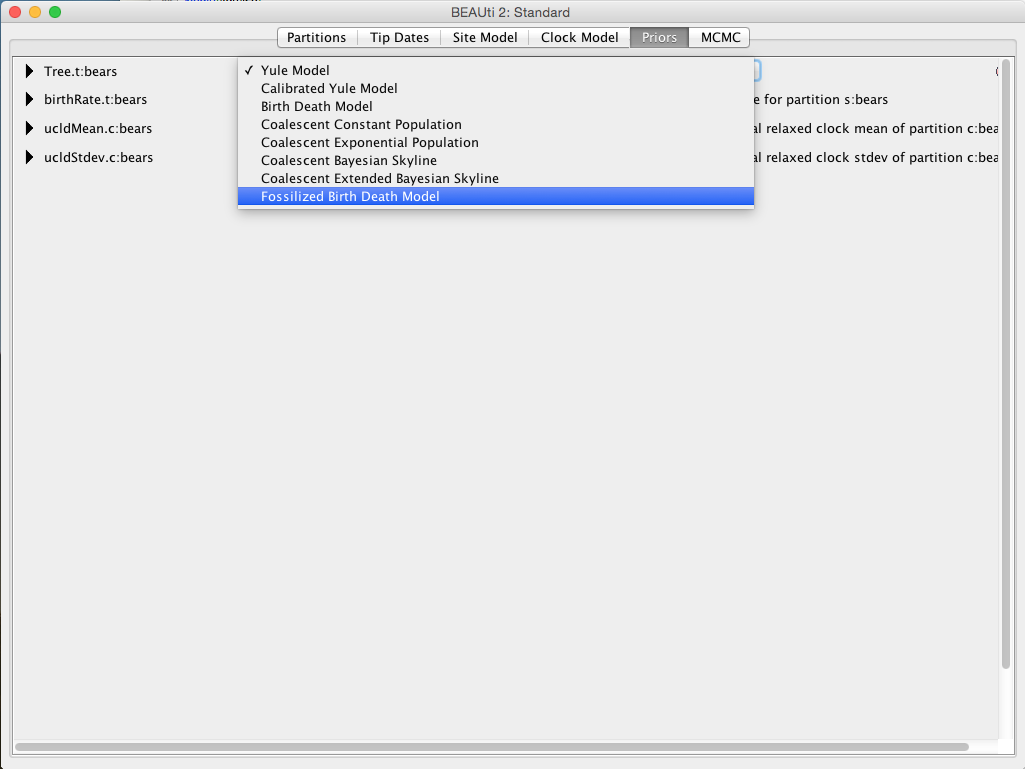
\includegraphics[width=\textwidth]{figures/FBDmodel}
\caption{Choose the `Fossilised Birth Death Model' in the {\bf Priors} panel. \label{fig:FBDmodel}}
\label{fig:BEAUti_ImportNexus}
\end{figure}

In the default settings of the FBD model, the proportion of species sampled at present, $\rho$, is fixed to one. For the example data we leave this setting. In other analyses, you might need to change this value depending on the sampling scheme. Also you might choose another parameter to be fixed or estimate all the parameters but place an informative prior on one or more. Although all the parameters in this model are identifiable, i.e., can be inferred from the phylogeny, in absence of comparative data of fossil samples we need to fix one of the parameters.  You might need to adjust the initial values of the parameters, e.g. time of origin, which has to be older than the oldest fossil sample. If you believe all the fossil samples are crown, that is the most recent common ancestor of all taxa included in the analysis is not a fossil or in other words the root of the phylogeny is a two-degree node and not a sampled node, then also tick `Condition on Root' box (see Figure \ref{fig:FBDsettings}). `Condition on Rho Sampling' is preferable for a dating analysis and we leave it selected. 

\begin{figure}	
\centering
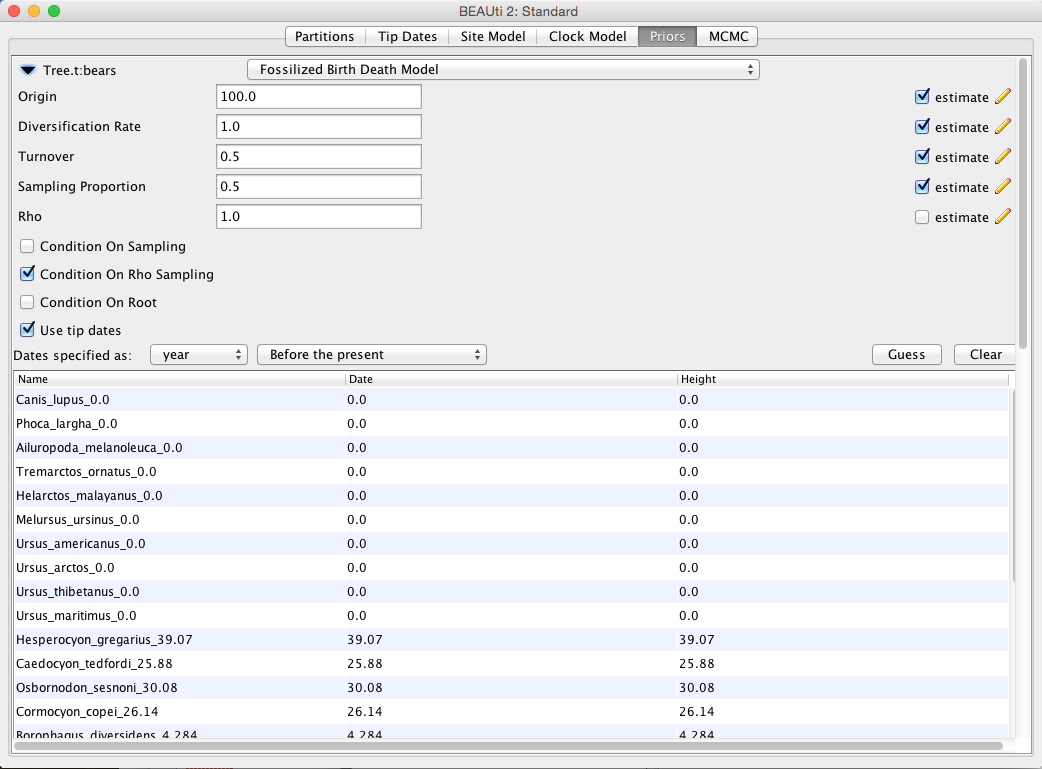
\includegraphics[width=\textwidth]{figures/FBDsettings}
\caption{The settings of the FBD model. All the parameter except for $\rho$ are estimated and $\rho$ is fixed to the one meaning that we sampled all the known species in the clade. We assume the most recent ancestor of all the taxa can be a fossil sample. So we do not select `Condition On Root'. \label{fig:FBDsettings}}
\label{fig:BEAUti_ImportNexus}
\end{figure}

Further, you may specify monophyletic constraints on the same panel. Click the plus button at the bottom of the {Priors} panel, name the monophyletic clade and select all the taxa included in the clade. Then tick the `monophyletic' box next to the `\#\#\#.prior' (\#\#\# is the name of the clade) and leave the prior distribution as `[none]' (see Figures \ref{fig:MonophyleticClade} and \ref{fig:MonophyleticConstraint}). We do not recommend to specify any distribution for internal nodes because the interaction between multiple distributions applied to the phylogeny is not well understood.
 
\begin{figure}	
\centering
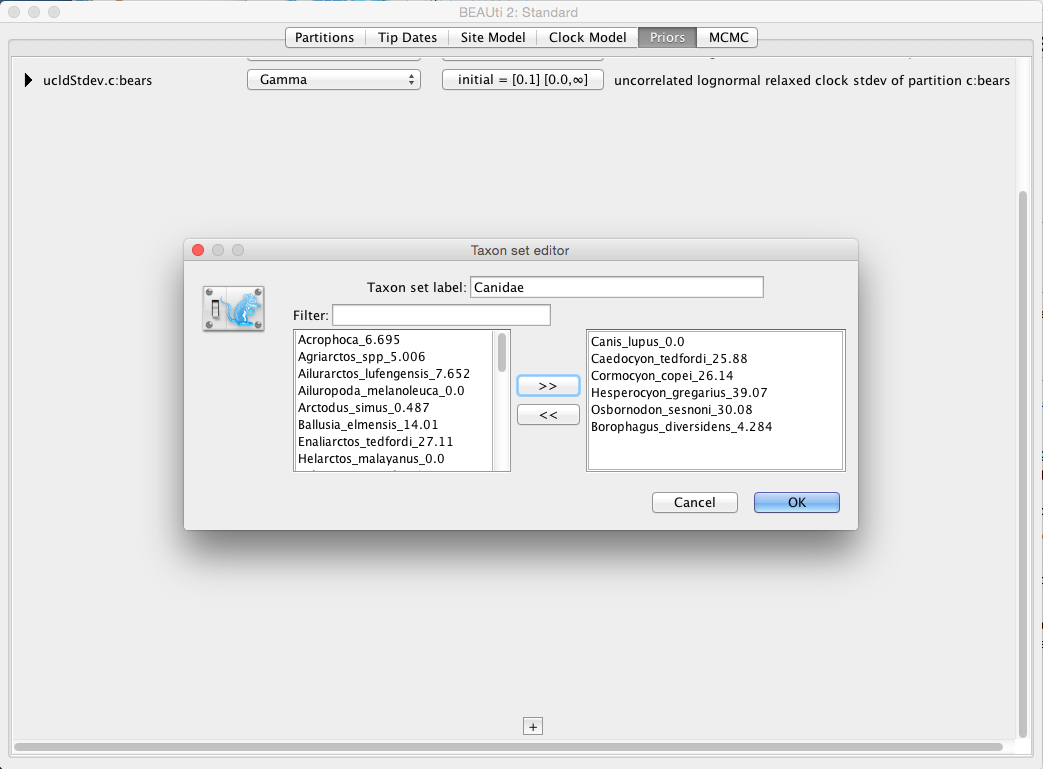
\includegraphics[width=\textwidth]{figures/MonophyleticClade}
\caption{Click the plus button at the bottom of the {\bf Priors} panel and specify the clade. Type in the name of the clade and put the clade members to the right box using arrow buttons. \label{fig:MonophyleticClade}}
\label{fig:BEAUti_ImportNexus}
\end{figure}

\begin{figure}	
\centering
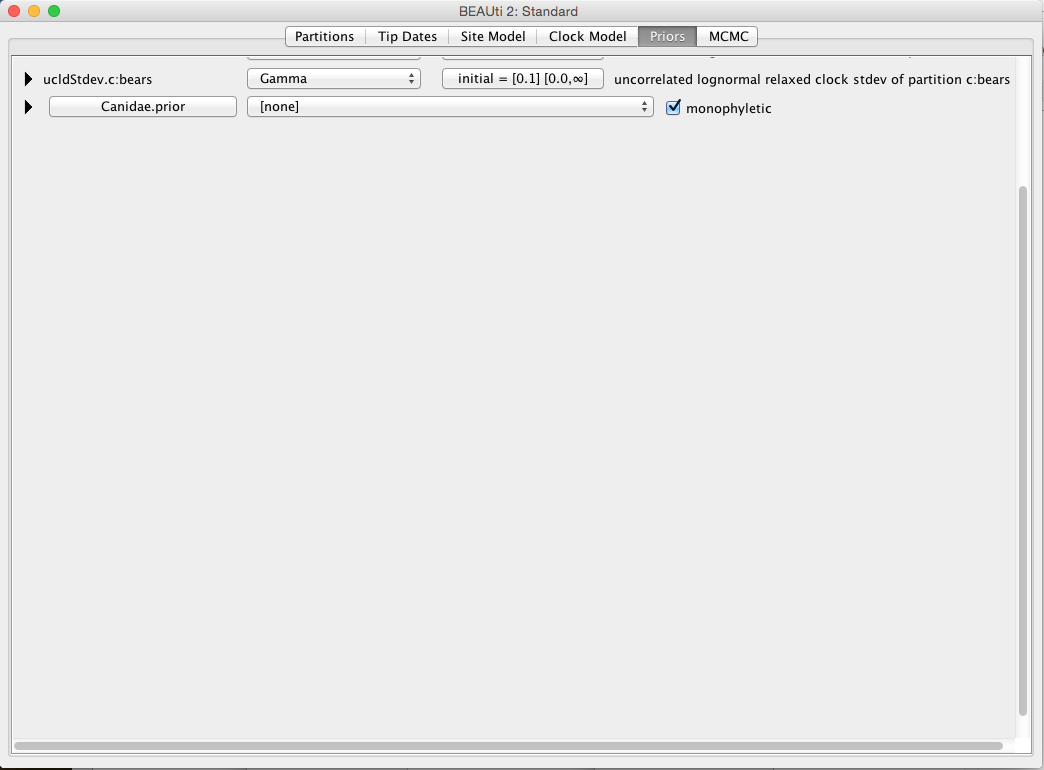
\includegraphics[width=\textwidth]{figures/MonophyleticConstraint}
\caption{Select monophyletic clade next to the clade prior. Leave the prior as `[none]'. \label{fig:MonophyleticConstraint}}
\label{fig:BEAUti_ImportNexus}
\end{figure}

Specify all the rest of the prior distribution and proceed with {\bf MCMC} panel. We only change the `Log Every' option for the `screenlog' to 10000 to make the output of BEAST analysis more compact. Then save the file. The resulting XML file, bears.xml, prepared following this tutorial can be found in {\tt examples/} in the SA package directory. 

Now the input XML file for BEAST is ready and you can run BEAST. 

\section{Analysing the results.} 

The output .log and .trees files will occur in the same directory where the XML file is. Useful information is reported to the screen output. See this for information about the data, citations, and suggestions to improve the operator performance.  

Open the LOG file in Tracer to review estimated statistics. For this analysis, the important parameters are the tree model parameters: origin, diversification rate, turnover and sampling proportion. Another statistic of interest is the sampled ancestor count (SAcountFBD) which is the number of fossils that are direct ancestors of other fossils or extant taxa. Figure~\ref{fig:TracerOutput} shows the estimates of the model parameters and the posterior distribution for the number of sampled ancestors. 

\begin{figure}	
\centering
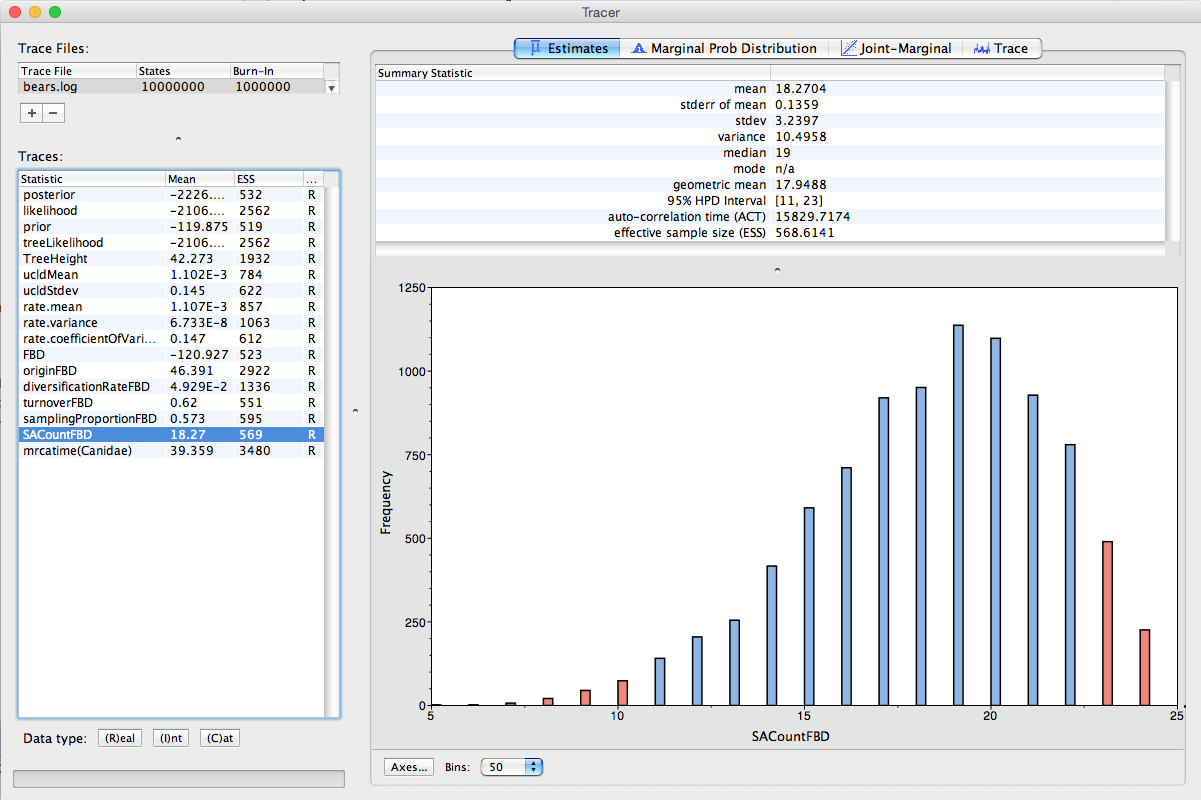
\includegraphics[width=\textwidth]{figures/TracerOutput}
\caption{The posterior estimates from the bear analysis in Tracer. \label{fig:TracerOutput}}
\end{figure}

Use TreeAnnotator to summarise the tree distribution and FigTree to view the summary tree. The summary tree of trees in bears.trees is shown in Figure~\ref{fig:FigTree}. It is obtained using TreeAnnotator with 10\% burnin, zero `Posterior probability limit', `Maximum Clade Credibility Tree' as the `Target tree type' and `Mean heights' as `Node heights'. To find the maximum clade credibility tree the TreeAnnotator takes into account sampled ancestor clades, that is, any two clades with the same taxa are considered as different clades if the most recent common ancestor in one clade is a sampled node and in another clade is a bifurcation node. The TreeAnnotator gives sensible results for sampled ancestor trees only in case when fossil ages are fixed.  

\begin{figure}	
\centering
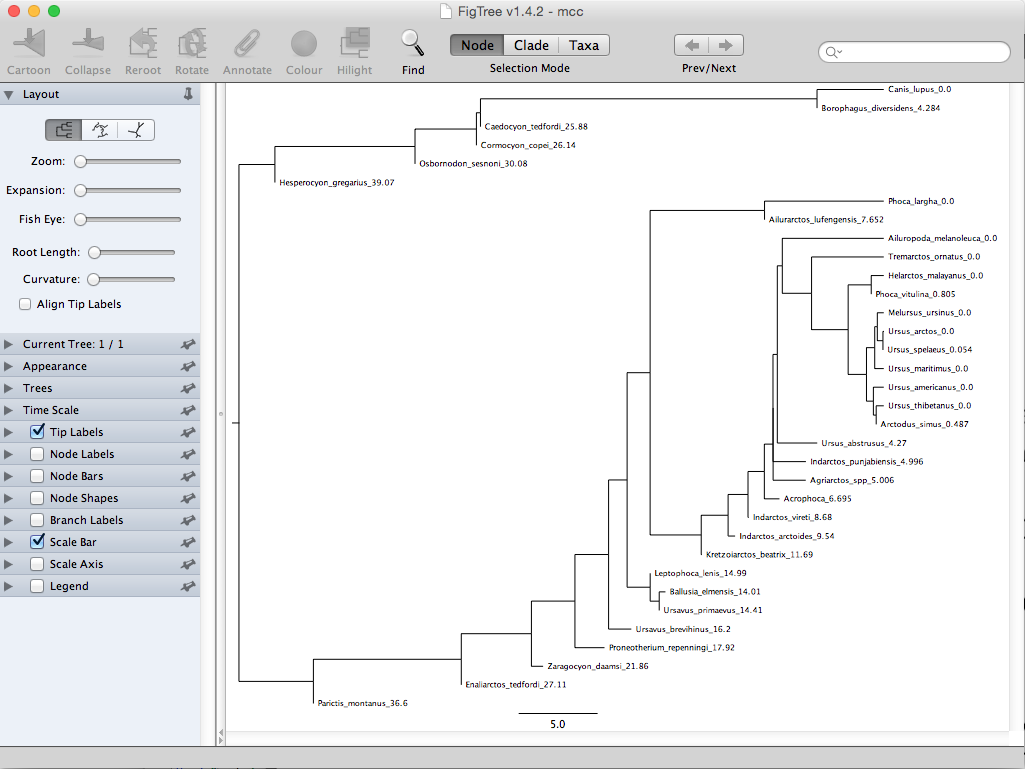
\includegraphics[width=\textwidth]{figures/FigTree}
\caption{FigTree view of the maximum clade credibility tree with mean node heights obtained with TreeAnnotator. The strictly horizontal branches (zero length branches) represent sampled ancestor nodes. \label{fig:FigTree}}
\end{figure}


%\bibliography{Total-evidenceWithSA}

\end{document}